\documentclass[11pt,twoside]{book}

\usepackage[utf8]{inputenc}

\usepackage{geometry}
\geometry{papersize={145mm,200mm}} % 60x84/16 is 145 mm x 200 mm
\geometry{tmargin=1.5cm,bmargin=1.5cm,lmargin=1.5cm,rmargin=1.5cm}

\usepackage{bm} % bold math symbols

\usepackage{amsmath}

\makeatletter
\newcommand{\raisemath}[1]{\mathpalette{\raisem@th{#1}}}
\newcommand{\raisem@th}[3]{\raisebox{#1}{$#2#3$}}
\makeatother

\makeatletter
\newcommand*\dotp{\mathpalette\dotp@{.55}}
\newcommand*\bigdot{\mathpalette\dotp@{.64}}
\newcommand*\dotp@[2]{\mathbin{\vcenter{\hbox{\scalebox{#2}{$\m@th#1\bullet$}}}}}
\makeatother
\newcommand\dotdotp{\dotp\hspace{-0.16em}\dotp\hspace{0.20em}}

\newcommand\onehalf{\raisemath{.02em}{\frac{\raisemath{-0.16em}{1}}{2}}}
\newcommand\smalldisplaystyleonehalf{\scalebox{0.8}{$\displaystyle \onehalf$}\hspace{.1ex}}

\newcommand\stiffnesstensorA{\hspace{.08ex}{^4\hspace{-0.72ex}\bm{\mathcal{A}}}\hspace{.08ex}}
\newcommand\stiffnesstensorB{{^4\hspace{-0.2ex}\bm{\mathcal{B}}}}
\newcommand\stiffnesstensorC{{^4\bm{\mathcal{C}}}}

\newcommand\stiffnesstensor{\stiffnesstensorA}
\newcommand\pliabilitytensor{\stiffnesstensorB}

\newcommand\expexternal{\raisemath{.1ex}{\smash{\hspace{.12ex}(\hspace{-0.1ex}e\hspace{-0.1ex})}\hspace{-0.16ex}}}
\newcommand\expinternal{\raisemath{.1ex}{\smash{\hspace{.12ex}(i)}\hspace{-0.16ex}}}

%%\newcommand\internalwork{W^{\hspace{-0.12ex}\expinternal}}
%%\newcommand\externalwork{W^{\hspace{-0.12ex}\expexternal}}

\usepackage{tikz}
\usetikzlibrary{calc}

\usepackage{upgreek}

\newcommand\variation[1]{\ensuremath\updelta\hspace{-0.1ex}#1}

\newcommand{\tikzsl}[1]{\tikz[baseline=(sl.base)] \node [xslant=0.21, inner sep=0pt, outer sep=0pt] (sl) {#1};}

\newcommand\mathboldtau{\scalebox{1}[1.06]{\tikzsl{\ensuremath{\bm{\uptau}\hspace{-0.1ex}}}}}

\newcommand\mathboldepsilon{\scalebox{1}[1.06]{\hspace{-0.2ex}\tikzsl{\scalebox{1.2}[1]{\ensuremath{\bm{\upvarepsilon}\hspace{-0.1ex}}}}}}

\pagestyle{empty}

\begin{document}

\begin{center}
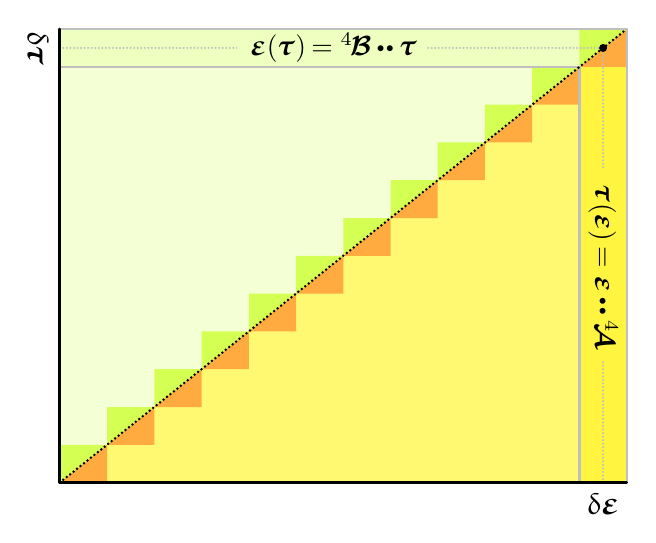
\begin{tikzpicture}[scale=0.72]

	\def\epsilonlength{10}
	\def\taulength{8}

	\fill [yellow!70!white, opacity=0.8] (0, 0) -- (\epsilonlength, \taulength) -- (\epsilonlength, 0) -- cycle ;
	\fill [lime!20!white, opacity=0.8] (0, 0) -- (\epsilonlength, \taulength) -- (0, \taulength) -- cycle ;

	\def\howmanysteps{12}
	\pgfmathsetmacro{\stepxlength}{\epsilonlength / \howmanysteps}
	\pgfmathsetmacro{\stepylength}{\taulength / \howmanysteps}
	\pgfmathsetmacro{\lastxstep}{\epsilonlength - \stepxlength}

	\foreach \xbox in { 0, \stepxlength, ..., \lastxstep }
	{
		\pgfmathsetmacro{\ybox}{\xbox * \taulength / \epsilonlength}
		\fill [orange!80!white, opacity=0.8]
			(\xbox, \ybox) -- (\xbox + \stepxlength, \ybox + \stepylength) -- (\xbox + \stepxlength, \ybox) -- cycle ;
		\fill [lime!80!white, opacity=0.8]
			(\xbox, \ybox) -- (\xbox + \stepxlength, \ybox + \stepylength) -- (\xbox, \ybox + \stepylength) -- cycle ;
	}

	\pgfmathsetmacro{\lastystep}{\taulength - \stepylength}
	\pgfmathsetmacro{\lastxboxmid}{\lastxstep + .5*\stepxlength}
	\pgfmathsetmacro{\lastyboxmid}{\lastystep + .5*\stepylength}

	\fill [yellow!75!white] (\lastxstep, 0) -- (\lastxstep, \lastystep) -- (\epsilonlength, \lastystep) -- (\epsilonlength, 0) -- cycle ;

	\draw [line width=0.8pt, color=black!25, line cap=round, dash pattern=on 0pt off 1.6\pgflinewidth]
		(\lastxboxmid, 0) -- (\lastxboxmid, \lastyboxmid)
		node [pos=0.5, rotate=-90, inner sep=1pt, outer sep=0pt, color=black, fill=yellow!75!white]
		{$\,\:\mathboldtau\hspace{.2ex}(\mathboldepsilon) \hspace{-0.2ex} = \mathboldepsilon \hspace{-0.1ex} \dotdotp \hspace{-0.1ex} \stiffnesstensor\;$} ;

	\draw [line width=0.8pt, color=black!25, line cap=round]
		(\lastxstep, 0) -- (\lastxstep, \lastystep) ;
	\draw [line width=0.8pt, color=black!25, line cap=round]
		(\epsilonlength, 0) -- (\epsilonlength, \taulength) ;
	\draw [line width=0.8pt, color=black!25, line cap=round]
		(\lastxstep, 0) -- (\epsilonlength, 0)
		node [pos=0.5, anchor=north, inner sep=0, outer sep=4pt, color=black]
		{\scalebox{1.1}[1.1]{$\variation{\mathboldepsilon}$}} ;

	\fill [lime!25!white] (0, \lastystep) -- (\lastxstep, \lastystep) -- (\lastxstep, \taulength) -- (0, \taulength) -- cycle ;

	\draw [line width=0.8pt, color=black!25, line cap=round, dash pattern=on 0pt off 1.6\pgflinewidth]
		(0, \lastyboxmid) -- (\lastxboxmid, \lastyboxmid)
		node [pos=0.5, inner sep=1pt, outer sep=0pt, color=black, fill=lime!25!white]
		{$\,\:\mathboldepsilon(\hspace{-0.1ex}\mathboldtau\hspace{.1ex}) \hspace{-0.2ex} = \pliabilitytensor \hspace{-0.1ex} \dotdotp \hspace{-0.1ex} \mathboldtau\;$} ;

	\draw [line width=0.8pt, color=black!25, line cap=round]
		(0, \lastystep) -- (\lastxstep, \lastystep) ;
	\draw [line width=0.8pt, color=black!25, line cap=round]
		(0, \taulength) -- (\epsilonlength, \taulength) ;
	\draw [line width=0.8pt, color=black!25, line cap=round]
		(0, \lastystep) -- (0, \taulength)
		node [pos=0.5, anchor=north, rotate=-90, inner sep=0, outer sep=4pt, color=black]
		{\scalebox{1.1}[1.1]{$\variation{\hspace{-0.1ex}\mathboldtau}$}} ;

	\fill [color=black] (\lastxboxmid, \lastyboxmid) circle ( 2pt ) ;

	\draw [line width=1pt, color=black, line cap=round]
		(0, 0) -- (\epsilonlength, 0) ;

	\draw [line width=1pt, color=black, line cap=round]
		(0, 0) -- (0, \taulength) ;

	\draw [line width=1pt, color=black, line cap=round, dash pattern=on 0pt off 1.6\pgflinewidth]
		(0, 0) -- (\epsilonlength, \taulength) ;

\end{tikzpicture}
\end{center}

\vspace{-2em}

\begin{equation*}\begin{array}{c}
\variation{\bigl( \hspace{-0.2ex} \mathboldtau \dotdotp \mathboldepsilon \bigr)} \hspace{-0.2ex}
= \mathboldtau \dotdotp \variation{\mathboldepsilon} + \variation{\hspace{-0.1ex}\mathboldtau} \dotdotp \mathboldepsilon
= \variation{\Pi} + \variation{\widehat{\Pi}}
\\[.3em]
%
\variation{\Pi} = \mathboldtau \dotdotp \variation{\mathboldepsilon}
= \mathboldepsilon \hspace{-0.1ex} \dotdotp \hspace{-0.1ex} \stiffnesstensor \hspace{-0.1ex} \dotdotp \variation{\mathboldepsilon} ,
\:\:
\variation{\widehat{\Pi}} = \variation{\hspace{-0.1ex}\mathboldtau} \dotdotp \mathboldepsilon
= \mathboldtau \hspace{-0.1ex} \dotdotp \hspace{-0.2ex} \pliabilitytensor \hspace{-0.1ex} \dotdotp \variation{\hspace{-0.1ex}\mathboldtau}
\end{array}\end{equation*}

%%\vspace{1em}

\begin{center}
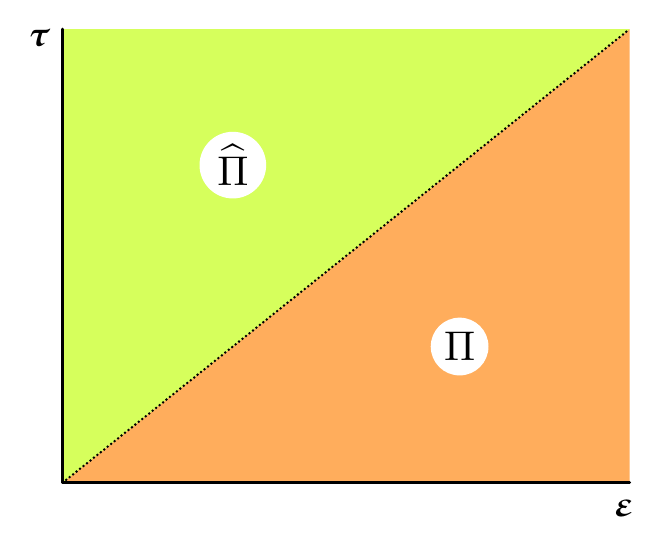
\begin{tikzpicture}[scale=0.72]

	\def\epsilonlength{10}
	\def\taulength{8}

	\fill [orange!80!white, opacity=0.8] (0, 0) -- (\epsilonlength, \taulength) -- (\epsilonlength, 0) -- cycle ;
	\fill [lime!80!white, opacity=0.8] (0, 0) -- (\epsilonlength, \taulength) -- (0, \taulength) -- cycle ;

	\draw [line width=1pt, color=black, line cap=round]
		(0, 0) -- (\epsilonlength, 0)
		node [pos=0.99, anchor=north, inner sep=0, outer sep=6pt]
		{\scalebox{1.2}[1.2]{$\mathboldepsilon$}} ;

	\draw [line width=1pt, color=black, line cap=round]
		(0, 0) -- (0, \taulength)
		node [pos=0.98, anchor=east, inner sep=0, outer sep=5pt]
		{\scalebox{1.2}[1.2]{$\mathboldtau$}} ;

	\draw [line width=1pt, color=black, line cap=round, dash pattern=on 0pt off 1.6\pgflinewidth]
		(0, 0) -- (\epsilonlength, \taulength) ;

	\draw (0.7 * \epsilonlength, 0.3 * \taulength) circle (0.1)
		node [color=black, anchor=center, shape=circle, fill=white, outer sep=5pt, inner sep=2pt]
		{\scalebox{1.5}[1.5]{$\Pi$}} ;

	\draw (0.3 * \epsilonlength, 0.7 * \taulength) circle (0.1)
		node [color=black, anchor=center, shape=circle, fill=white, outer sep=5pt, inner sep=2pt]
		{\scalebox{1.5}[1.5]{$\widehat{\Pi}$}} ;

\end{tikzpicture}
\end{center}

\vspace{-2em}

\begin{equation*}\begin{array}{c}
\mathboldtau \dotdotp \mathboldepsilon
= \hspace{.1ex}
\Pi(\mathboldepsilon) \hspace{-0.1ex} + \hspace{.1ex} \widehat{\Pi}(\hspace{-0.1ex}\mathboldtau\hspace{.12ex}) \hspace{-0.1ex}
\\[.4em]
%
\Pi(\mathboldepsilon) \hspace{-0.1ex}
= \smalldisplaystyleonehalf \hspace{.2ex} \mathboldtau\hspace{.2ex}(\mathboldepsilon) \hspace{-0.2ex} \dotdotp \mathboldepsilon
= \smalldisplaystyleonehalf \hspace{.25ex} \mathboldepsilon \hspace{-0.1ex} \dotdotp \hspace{-0.1ex} \stiffnesstensor \hspace{-0.1ex} \dotdotp \mathboldepsilon
\\[.4em]
%
\widehat{\Pi}(\hspace{-0.1ex}\mathboldtau\hspace{.12ex}) \hspace{-0.1ex}
= \smalldisplaystyleonehalf \hspace{.2ex} \mathboldtau \dotdotp \mathboldepsilon(\hspace{-0.1ex}\mathboldtau\hspace{.12ex}) \hspace{-0.1ex}
= \smalldisplaystyleonehalf \hspace{.15ex} \mathboldtau \hspace{-0.1ex} \dotdotp \hspace{-0.2ex} \pliabilitytensor \hspace{-0.1ex} \dotdotp \hspace{-0.1ex} \mathboldtau
\end{array}\end{equation*}

\end{document}
